%%%%%%%%%%%%%%%%%%%%%%%%%%%%%%%%%%%%%%%%%
% Wenneker Article
% LaTeX Template
% Version 2.0 (28/2/17)
%
% This template was downloaded from:
% http://www.LaTeXTemplates.com
%
% Authors:
% Vel (vel@LaTeXTemplates.com)
% Frits Wenneker
%
% License:
% CC BY-NC-SA 3.0 (http://creativecommons.org/licenses/by-nc-sa/3.0/)
%
%%%%%%%%%%%%%%%%%%%%%%%%%%%%%%%%%%%%%%%%%

%----------------------------------------------------------------------------------------
%	PACKAGES AND OTHER DOCUMENT CONFIGURATIONS
%----------------------------------------------------------------------------------------

\documentclass[10pt, letterpaper, twocolumn]{article} % 10pt font size (11 and 12 also possible), A4 paper (letterpaper for US letter) and two column layout (remove for one column)

%%%%%%%%%%%%%%%%%%%%%%%%%%%%%%%%%%%%%%%%%
% Wenneker Article
% Structure Specification File
% Version 1.0 (28/2/17)
%
% This file originates from:
% http://www.LaTeXTemplates.com
%
% Authors:
% Frits Wenneker
% Vel (vel@LaTeXTemplates.com)
%
% License:
% CC BY-NC-SA 3.0 (http://creativecommons.org/licenses/by-nc-sa/3.0/)
%
%%%%%%%%%%%%%%%%%%%%%%%%%%%%%%%%%%%%%%%%%

%----------------------------------------------------------------------------------------
%	PACKAGES AND OTHER DOCUMENT CONFIGURATIONS
%----------------------------------------------------------------------------------------

\usepackage[english]{babel} % English language hyphenation

\usepackage{microtype} % Better typography

\usepackage{amsmath,amsfonts,amsthm} % Math packages for equations

\usepackage[svgnames]{xcolor} % Enabling colors by their 'svgnames'

\usepackage[hang, small, labelfont=bf, up, textfont=it]{caption} % Custom captions under/above tables and figures

\usepackage{booktabs} % Horizontal rules in tables

\usepackage{lastpage} % Used to determine the number of pages in the document (for "Page X of Total")

\usepackage{graphicx} % Required for adding images

\usepackage{enumitem} % Required for customising lists
\setlist{noitemsep} % Remove spacing between bullet/numbered list elements

\usepackage{sectsty} % Enables custom section titles
\allsectionsfont{\usefont{OT1}{phv}{b}{n}} % Change the font of all section commands (Helvetica)

%----------------------------------------------------------------------------------------
%	MARGINS AND SPACING
%----------------------------------------------------------------------------------------

\usepackage{geometry} % Required for adjusting page dimensions

\geometry{
	top=1cm, % Top margin
	bottom=1.5cm, % Bottom margin
	left=2cm, % Left margin
	right=2cm, % Right margin
	includehead, % Include space for a header
	includefoot, % Include space for a footer
	%showframe, % Uncomment to show how the type block is set on the page
}

\setlength{\columnsep}{7mm} % Column separation width

%----------------------------------------------------------------------------------------
%	FONTS
%----------------------------------------------------------------------------------------

\usepackage[T1]{fontenc} % Output font encoding for international characters
\usepackage[utf8]{inputenc} % Required for inputting international characters

\usepackage{XCharter} % Use the XCharter font

%----------------------------------------------------------------------------------------
%	HEADERS AND FOOTERS
%----------------------------------------------------------------------------------------

\usepackage{fancyhdr} % Needed to define custom headers/footers
\pagestyle{fancy} % Enables the custom headers/footers

\renewcommand{\headrulewidth}{0.0pt} % No header rule
\renewcommand{\footrulewidth}{0.4pt} % Thin footer rule

\renewcommand{\sectionmark}[1]{\markboth{#1}{}} % Removes the section number from the header when \leftmark is used

%\nouppercase\leftmark % Add this to one of the lines below if you want a section title in the header/footer

% Headers
\lhead{} % Left header
\chead{\textit{\thetitle}} % Center header - currently printing the article title
\rhead{
\includegraphics{../images/logo_block}} % Right header

% Footers
\lfoot{} % Left footer
\cfoot{} % Center footer
\rfoot{\footnotesize Page \thepage\ of \pageref{LastPage}} % Right footer, "Page 1 of 2"

\fancypagestyle{firstpage}{ % Page style for the first page with the title
	\fancyhf{}
	\renewcommand{\footrulewidth}{0pt} % Suppress footer rule
	%\renewcommand{\headheight}{12pt}
}

%----------------------------------------------------------------------------------------
%	TITLE SECTION
%----------------------------------------------------------------------------------------

\newcommand{\authorstyle}[1]{{\large\usefont{OT1}{phv}{b}{n}\color{MidnightBlue}#1}} % Authors style (Helvetica)

\newcommand{\institution}[1]{{\footnotesize\usefont{OT1}{phv}{m}{sl}\color{Black}#1}} % Institutions style (Helvetica)

\usepackage{titling} % Allows custom title configuration

\newcommand{\HorRule}{\color{CornflowerBlue}\rule{\linewidth}{1pt}} % Defines the gold horizontal rule around the title

\pretitle{
	\vspace{-30pt} % Move the entire title section up
	\HorRule\vspace{10pt} % Horizontal rule before the title
	\fontsize{24}{26}\usefont{OT1}{phv}{b}{n}\selectfont % Helvetica
	\color{MidnightBlue} % Text colour for the title and author(s)
}

\posttitle{\par\vskip 15pt} % Whitespace under the title

\preauthor{} % Anything that will appear before \author is printed

\postauthor{ % Anything that will appear after \author is printed
	\vspace{0pt} % Space before the rule
	\par\HorRule % Horizontal rule after the title
	\vspace{0pt} % Space after the title section
}

%----------------------------------------------------------------------------------------
%	ABSTRACT
%----------------------------------------------------------------------------------------

\usepackage{lettrine} % Package to accentuate the first letter of the text (lettrine)
\usepackage{fix-cm}	% Fixes the height of the lettrine
\usepackage{hyperref}	% Fixes the height of the lettrine

\newcommand{\initial}[1]{ % Defines the command and style for the lettrine
	\lettrine[lines=3,findent=4pt,nindent=0pt]{% Lettrine takes up 3 lines, the text to the right of it is indented 4pt and further indenting of lines 2+ is stopped
		\color{Grey}% Lettrine colour
		{#1}% The letter
	}{}%
}

\usepackage{xstring} % Required for string manipulation

\newcommand{\lettrineabstract}[1]{
	\StrLeft{#1}{1}[\firstletter] % Capture the first letter of the abstract for the lettrine
	\initial{\firstletter}\textbf{\StrGobbleLeft{#1}{1}} % Print the abstract with the first letter as a lettrine and the rest in bold
}

%----------------------------------------------------------------------------------------
%	BIBLIOGRAPHY
%----------------------------------------------------------------------------------------

\usepackage[backend=bibtex,style=authoryear,natbib=true]{biblatex} % Use the bibtex backend with the authoryear citation style (which resembles APA)

\addbibresource{example.bib} % The filename of the bibliography

\usepackage[autostyle=true]{csquotes} % Required to generate language-dependent quotes in the bibliography
 % Specifies the document structure and loads requires packages
\usepackage{titling}
\usepackage{graphicx}

\usepackage{fancyhdr}
\pagestyle{fancy}

\usepackage{xcolor}

\usepackage{lipsum}
\setlength\headheight{20pt} %% just to make warning go away. Adjust the value after looking into the warning.
% \rhead{{\color{blue}\rule{1cm}{1cm}}}

\rhead{
\includegraphics[width=2cm]{../images/logo_block}}

%----------------------------------------------------------------------------------------
%	ARTICLE INFORMATION
%----------------------------------------------------------------------------------------
\pretitle{%
  \begin{center}
  \LARGE
  
\includegraphics[width=3.43cm,height=2.26cm]{../images/logo_block}\\
}
\posttitle{\end{center}}

\title{Quantitative Virology and Evolution Unit Laboratory Manual} % The article title

\author{
	\authorstyle{Patrick T. Dolan, Ph.D.\textsuperscript{1}} % Authors
	\newline % Space before institutions
	\textsuperscript{1}\institution{Unit Chief, Quantitative Virology and Evolution Unit, Laboratory of Viral Diseases, NIH-NIAID, Bethesda, MD, United States of America}\\ % Institution 1
}

% Example of a one line author/institution relationship
%\author{\newauthor{John Marston} \newinstitution{Universidad Nacional Autónoma de México, Mexico City, Mexico}}

\date{\today} % Add a date here if you would like one to appear underneath the title block, use \today for the current date, leave empty for no date

%----------------------------------------------------------------------------------------

\begin{document}

\maketitle % Print the title

\thispagestyle{firstpage} % Apply the page style for the first page (no headers and footers)

%----------------------------------------------------------------------------------------
%	ABSTRACT
%----------------------------------------------------------------------------------------

\lettrineabstract{The purpose of this document is to lay out general expectations and provide information for members of the Quantitative Virology and Evolution Unit (QVEU). This is a living document that will change as the lab changes. Please read it thoroughly. If anything in this document seems incorrect, outdated, or you think a process or policy can be improved, please bring it up to Patrick or the group. Even though this is not a permanent document, it is important that we all agree to follow the expectations as defined here and respect the process as it’s set forth.}

%----------------------------------------------------------------------------------------
%	ARTICLE CONTENTS
%----------------------------------------------------------------------------------------

\section{Introduction}
\subsection{Welcome}
Welcome to the \href{http://qveu.github.io/QVEU/}{Quantitative Virology and Evolution Unit} (A.K.A., the Dolan Lab) in the \href{https://www.niaid.nih.gov/research/lab-viral-diseases}{Laboratory of Viral Diseases} at NIH. Whether you are a student, fellow, or staff member, I am incredibly honored and excited that you’ve chosen to continue your scientific work here. I look forward to supporting your development as a scientist, and look forward to learning with and from you during your time in the lab.

\subsection{The Mission}
The mission of the QVEU is to explore questions related to virus evolution, emergence, and pathogenesis through rigorous quantitative experiments and computational biology.

The three concepts I want to motivate the lab are:
\begin{description}
	\item [Heterogeneity] - how does diversity and selection in viral and host cell populations affect the outcome of infection and evolution?
	\item [Constraint] - what are the forces (biological, genetic, or biophysical) that shape evolutionary processes?
	\item [History] - how can historical data (either measured or inferred computationally) be used to enhance our understanding of viral diversification and emergence?
\end{description}
\subsection{Motivating Values}
Core values are the beliefs that motivate us. In my scientific training, I’ve found my two core values are Curiosity and Responsibility. To me, scientific curiosity is the fuel that runs this machine. Without it, we have no new questions and can easily find ourselves just “punching the clock” and doing the same experiments on the same variables we always have. When things aren’t working, it is my own curiosity that will keep me asking new questions and spurring me on through the difficult times. Responsibility is what makes us do the rest of the job - the paperwork, cleaning, organization, and participation - when we might rather not. I encourage you to think about your own core values and how they motivate you and shape your interactions. My core values shape this document. I also want to understand how your core values motivate you.
\subsection{Setting: The LVD, NIAID, and the NIH}
The Quantitative Virology and Evolution Unit is part of the Laboratory of Viral Diseases (the LVD). The LVD operates under the Division of Intramural Research, the intramural reseearch arm of the National Institute of Allergy and Infectious Diseases (NIAID). NIAID is one of Institutes that makes up the National Institutes of Health (the NIH).

To put it in terms of academia, you could think of the LVD as your "Department", the Lab Chief as the Department Chair, and the NIAID Division of Intramural Research ("the DIR") as your college.

\begin{figure}
	
\includegraphics[width=\linewidth]{unitlab.png} % Figure image
	\caption{Diagram of NIH organizational structure. From the very helpful \href{https://www.training.nih.gov/assets/2019_Postbac_Handbook_Accessible.pdf}{Post-bac handbook.}} % Figure caption
	\label{unit_organization} % Label for referencing with \ref{bear}
\end{figure}

\section{General Lab Information}
\subsection{Contact Information}
\begin{description}
\item [Lab Address]: \newline Building 33, Room 1E19 \newline 33 North Drive, MSC 3210 \newline Bethesda, MD 20892-3210
\item [Patrick's Cell Phone]: 989-600-0117
\item [Patrick's Office Phone]: 301-761-7533
\end{description}

\subsection{Important Contact Numbers}
\begin{description}
\item [Building Maintenance Requests:] 301-435-8000 or \href{https://www.orf.od.nih.gov/PropertyManagement/MaintenanceServiceRequests/Pages/default.aspx}{on the NIH intranet}
\item [NIAID IT Help Tickets:]
\href{mailto:niaidithelp@niaid.nih.gov}{niaidithelp@niaid.nih.gov}
\item [Building 33 staff:] \href{mailto:33LANSTAFF@niaid.nih.gov}{33LANSTAFF@niaid.nih.gov}
\item [Office of Research Training and Development:]
Email: niaidtraining@nih.gov\newline
Phone: 1 (301) 761-5673
\item [USPS Mail Delivery Service:] 301-496-3586
\end{description}

\section{Onboarding Tasks}
Here is a brief outline of what to expect once you have received an offer to join the lab. Because we are a government lab, and because our building requires special clearance, there are a few extra steps that will be required, especially if you are planning to do any BSL3 work.
NOTE: If you are planning, or might plan, to do any BSL3 work, we should discuss this and make sure the admin team knows.

\subsection{After accepting your offer}
\begin{enumerate}
\item Receive initial e-mail from LVD Admin team and complete LVD paperwork.
\item Complete DPSAC background check through eQIP.
\item Get fingerprints recorded at NIH or at a remote office (this will accelerate things with DPSAC).
\item You will be activated in NED NIH Directory system on your start date.
\item Set up "PIV card" badging and issuance appointments at NIH security office (Bldg. 31).
\item Get badge access to the building activated, Patrick or LVD admins must request from Authorizing Official (AO).
\item Get VPN access to NIH systems so you can access trainings and other NIH services.
\end{enumerate}

\subsection{Once you have your badge and computer}
Complete NIH mandated trainings. Some of these will be role and project specific. Overall trainees and FTEs have different requirements (some are required for all).  Trainees will learn about required training in the mandatory NIAID ORTD Orientation.
The trainings have various due dates, but try to finish in first two weeks:
\begin{description}
\item[Information Security and Information Management:]\href{https://irtsectraining.nih.gov/}{https://irtsectraining.nih.gov/}
\item[Lab Safety:]\href{https://www.safetytraining.nih.gov/}{https://www.safetytraining.nih.gov/}
\item[Bloodborne Pathogens Training:]\href{https://www.safetytraining.nih.gov/}{https://www.safetytraining.nih.gov/}
\item[AMBIS for requesters:] Short course on how to place order requests. \href{https://lms.learning.hhs.gov/Saba/Web_wdk/Main/learning/learningOfferingDetails.rdf}{link in LMS}
\item[Government Ethics Training:]\href{https://researchethics.od.nih.gov/}{https://researchethics.od.nih.gov/}
\item[Animal Training:]Required for anyone listed on Animal Safety Protocol (ASP) \href{https://oacutraining.od.nih.gov/default.aspx}{https://oacutraining.od.nih.gov/default.aspx}. All animal users must also read and understand all of the items listed in the ASP.
\item[Anti-harrassment Training:]\href{https://www.edi.nih.gov/training/mandatory-training}{https://www.edi.nih.gov/training/mandatory-training}
\item[Responsible Conduct of Research, Annual Case Studies:] Search  "\%RCR\%"" on the Learning Management System (LMS) \href{https://lms.learning.hhs.gov/}{https://lms.learning.hhs.gov/}. See this link for more info on ethical requirments \href{https://oir.nih.gov/sourcebook/ethical-conduct/responsible-conduct-research-training}{https://oir.nih.gov/sourcebook/ethical-conduct/responsible-conduct-research-training}
\end{description}

\subsection{Once you are in lab}
\begin{enumerate}
\item Get necessary software (see "Software") installed on your Government-issued device.
\item Complete lab tour and orientation.	Learn where things are, how things work, where to order, where to shop on campus for equipment and reagents.
\item Complete computational orientation. Learn the basics of GitHub Desktop and Atom, R, and python. Start by editing your lab website entry!
\item Get access to storage space and Locus High-Performance Cluster (HPC), learn how to submit jobs. Our lab group has been set up with an initial quota of 20TB. To request an account and access to our shared drive, \href{https://locus.niaid.nih.gov/userportal/documentation.php#Getting-Started/Request-an-Account}{see instructions here.} More information and tutorials are \href{https://locus.niaid.nih.gov}{here.}
\end{enumerate}

\section{Expectations}
\subsection{Lab Policies}
It is my responsibility to provide you with a safe, supportive, and productive environment for you to work, train, and study. I hope all lab members will become active participants in creating a lab culture of curiosity, rigor, and shared success. These are a few expectations I hope will provide a substrate on which that culture can grow.

\subsubsection{Working Hours}
There are no specific "working hours" for the lab, but official lab activities will operate on a 9-to-5 schedule. This means lab meetings, discussion, 1-on-1's, seminars, and trainings will be scheduled between 9AM and 5PM, Monday through Friday. Schedules are sometimes irregular due to experimental timelines, variable workloads, equipment schedules, or commitments at home. You can keep a schedule that works for you as long as you are productive and you attend the scheduled lab meetings. If there is an important conflict with the scheduled lab events, we will find a new time that works for all lab members. The lab will not close on weekends, but I do expect you will use your weekends to recharge for the week as needed.

\subsubsection{Working remotely} Working remotely is sometimes conducive to completing a writing or coding task, but being in the lab helps to foster communication, coordination, and creativity through organic conversation between lab members and others on the NIH campus. Working remotely is a privilege and not a right. All members of the lab are expected to be in the lab for all lab meetings and seminars. {\bfseries COVID-19 note:} The unique situation presented by COVID-19 means that remote work will be a necessary part of the lab indefinitely. It is critical that we prioritize the wet-lab work onsite, and perform writing and coding projects off-site as necessary. This will require extra coordination and organization across the lab group. We will rely on the lab Slack and other scheduling tools as necessary to facilitate this coordination.

\subsubsection{Lab absences} If you expect to be out of the lab for more than a day, please put this on the lab calendar along with whether you are available to be contacted. You can also put up a status on Slack. This helps everyone know not to bother you (except in an emergency), or to store deliveries that may need special handling.

\subsubsection{Illness} You should make every effort to avoid coming to lab if you have a contagious illness. Contact your labmates to cover for you, if necessary. If you do need to come to work for an urgent reason, minimize contact with your co-workers, wear a mask, and wash your hands regularly to avoid transmission.

\subsubsection{Vacation} I expect you to take advantage of the weekends and vacation time you have. I want you to balance your mental health and well-being with your productivity. Please do your best to plan vacations around important deadlines and give yourself and your collaborators ample time to plan ahead.

\subsubsection{Language}
Since English will be the language we use to write and present our work, please speak and write in English in the lab and office with your colleagues and coworkers. It is important to avoid misunderstandings, facilitate interactions, and prevent isolation. It also gives those for whom English is not a first language more opportunities to practice speaking about their work in English.

\subsubsection{Dress code} There is no dress code beyond any set forth by the NIH, but you should be presentable when on campus and dress with safety in mind. Closed-toe shoes and long pants are required in the lab, long hair should be tied back, loose clothing or dangling jewelry should be avoided. There are lockers available for those who may want to change into lab clothes, lab shoes, or scrubs prior to work. You can request a locker with the LVD admin team when you arrive on campus.

\subsubsection{Food/drink} Food and drink are banned from lab bench areas. Do not store food in the office area, and do not leave any empty containers or food waste anywhere in the office area. You are welcome to use the fridge in the lunch room, the entry lobby, or in Patrick's office.

\subsubsection{Professionalism}
Punctuality is expected at lab meetings and seminars. All members of the lab are to treat others with respect inside and outside of the lab. When representing the lab at a conference, symposium, or NIH function, lab members are expected to exhibit behavior that exemplifies our values.

\subsubsection{Discrimination and Harassment}
Abuse, harassment, or discriminatory behavior of any kind will not be tolerated. It is my priority that this lab be an example of tolerance, compassion, and acceptance. No one will be treated differently due to the race, color, religion, sexual orientation, gender, socioeconomic background, or any other reason. I ask that everyone respect the boundaries of their labmates. We will not tolerate the display of racist or offensive signs or images; offensive jokes based on race, gender or other grounds that result in awkwardness, embarrassment or unwelcome attention.

\subsubsection{Lab maintenance and repairs}
Working at the NIH is a tremendous privilege and it is critical that we treat the taxpayers' lab and equipment with respect. It is also critical to your work, the work of your colleagues in the lab, and that of our neighbors in the LVD that we maintain our equipment in excellent condition. Any broken or malfunctioning equipment should be discussed as soon as possible, preferably by the party who discovered the issue.
In order to encourage the maintenance of the lab in good working order, the lab will have a shutdown each spring where we thoroughly clean, declutter, and inventory the lab and any equipment that requires repair, replacement, or to be sent to surplus can be identified. We will also regularly clean the lab space with 5\% bleach and then 70\% ethyl/isopropyl alcohol.

\subsubsection{Being a good lab citizen}
Science is sometimes difficult, but made easier through the support of our labmates. I want members of the lab to be generous with their time, resources, and expertise. I expect you to participate in group meetings, give constructive feedback, ask questions, suggest experiments, offer assistance, and generally support the work of your labmates. You should expect the same of them. We should be understanding of others' working styles and, when possible, flex to work with them in a way that they are comfortable. I want us all to build a culture of shared success and not one of intra-lab competition.

\subsubsection{Conflict Resolution}
Working together for years, sometimes under pressure, in small spaces can naturally lead to disagreements and conflicts. As adults, we should all be willing to be deal with issues directly, professionally, and honestly. We should also be aware and understanding of others' boundaries, preferences, and customs, and avoid issues where possible. When serious interpersonal issues arise in the QVEU or LVD, they should be brought to Patrick's attention as soon as possible.

\subsubsection{Criticism}
Criticism and feedback are an important part of the scientific process. It improves our work and forces us to think from new perspectives. The ability to give and receive feedback effectively is an essential scientific skill, but requires trust between team members. To encourage that trust, we must always give criticism in a thoughtful and constructive way. I understand not all members of the lab may be comfortable giving and receiving feedback or criticism in the same way, so I encourage you to find and communicate an approach that works for you.

\subsubsection{Mistakes}
Mistakes are a natural part of learning, but making the same mistake is not. I want everyone to own up to their mistakes so that they and others can learn from them and we can take any steps possible to avoid them in the future.

\subsubsection{Safety}
As virologists, the work we do has some inherent risks, which we minimize through building (engineering) controls, specialized equipment, and specific training in safe practices. It is critical that we all observe key safety rules to keep us all safe and compliant.\newline \newline
{\bfseries Situational awareness} is the key to safety. Everyone is expected to exercise situational awareness in the lab.

\begin{description}
\item [Perception] - of the elements in the environment
\item [Comprehension] - of the situation
\item [Projection] - of future status
\end{description}
Some general safety guidelines for the lab (Adapted from Safety in a Microbiological Laboratory, CDC guidance \citep{US_Department_of_Health_and_Human_Services2020-ck}):
\begin{enumerate}
	\item Hygiene:
	\begin{description}
		\item Wash your hands coming in and going out of the lab and between tasks.
		\item Do not eat or drink in lab area.
		\item Isolate your lab surfaces from your computers and personal devices in the office area.
		\end{description}
	\item Equipment:
		\begin{description}
		\item Do you have the necessary equipment and PPE to do the experiment safely? Think about this far ahead of time so we can get what you need.
		\item Appropriate equipment for the job?
		\item Reduce risk where possible.
		\item Minimize splashing and aerosolization.
		\item Secondary containment when necessary.
		\end{description}
	\item Decontamination:
		\begin{description}
		\item Clean work surfaces.
		\item Place all contaminated items in leak-proof containers.
		\item Use secondary containment when transporting infectious materials (e.g. a locked, plastic container to hold your tube rack).
		\item Regular decontamination is critical to high quality work. We will keep a tidy, decontaminated work area (regularly 10\% bleach, water, and 70\% Ethanol).
		\item Be aware of what come into the work area and what goes out.
		\end{description}
	\item Signs and Labels:
		\begin{description}
		\item	Make sure you are working in designated areas appropriately.
		\item Make sure your work area, reagents and waste are appropriately labeled.
		\end{description}
	\item Training:
		\begin{description}
		\item Are you properly trained to use a piece of equipment?
		\item Have you done adequate preparation (i.e. reading), planning, and visualization to foresee potential risks?
		\end{description}
\end{enumerate}
If you do not know the appropriate {\it hygiene, equipment, decontamination or labeling} necessary for a given task, you still require some {\it training}. That’s OK, just ask!

\begin{figure*}
  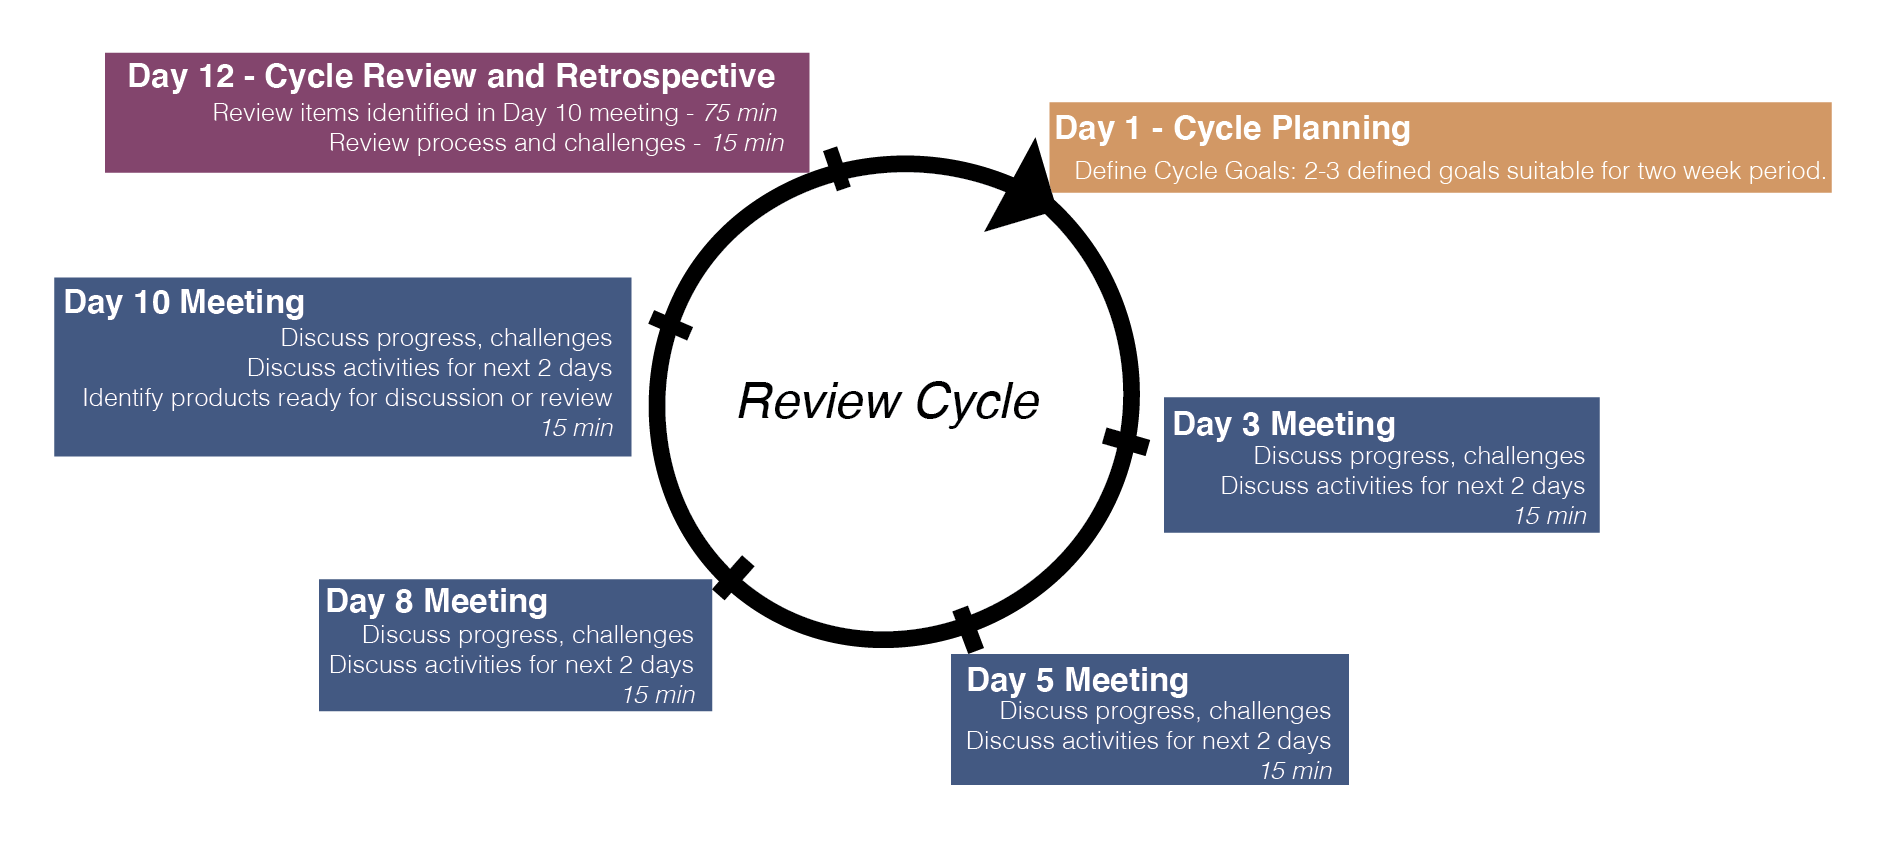
\includegraphics[width=\textwidth]{Core_Competencies-02.png}
  \caption{Biweekly cycle schedule.}
\end{figure*}
\subsection{Lab Meetings}
Traditional lab meeting and journal club models are not always effective at engaging and encouraging participation.  In addition, our lab is small and we are just getting started so there will be a lot of troubleshooting and optimization. Therefore, we are going to experiment with a modified version of the "Scrum" or "Agile" project management style \citep{May2019-kp} which will encourage effective and efficient communication. This will probably take a few months to get right, but we will improve it together.

In this framework, work is broken into "cycles" of some length of time (e.g. 2-3 weeks). At the beginning of each cycle each individual in the lab, including the PI, chooses goals for that cycle (2-3 goals appropriate to the cycle length) that are part of their larger project. Then, the team will meet regularly (every 2-3 days) to discuss their progress and identify any challenges in short, 15 minute meetings. At the final short meeting in a cycle (Day 10), the team will nominate items to be discussed at the "Cycle Review". Cycle Review is a more formal 90 minute meeting where we discuss the nominated results, manuscripts, recent publications, or practice presentations in more depth (more like a traditional lab meeting). At each Cycle Review, we will also have a Cycle Retrospective where we will evaluate any challenges we encountered and discuss whether the process itself can be improved or adapted to better suit our needs.

\begin{table*}
	\caption{Current cycle schedule}
	\centering
	\begin{tabular}{lll}
		\toprule
		\cmidrule(r){1-2}
		Day & Time Limit & Description \\
		\midrule
		M Day 1 & 30min & Cycle Planning - Set 2-3 goals for that 12 day cycle. \\
		W Day 3 & 15min & Cycle Meeting  \\
		F Day 5 & 15min & Cycle Meeting \\
		M Day 8 & 15min & Cycle Meeting \\
		W Day 10 & 15min & Cycle Meeting - Nominate any projects for review, either due to progress or challenges.  \\
		F Day 12 & 90min & Cycle Review and Retrospective \\
		\bottomrule
	\end{tabular}
\end{table*}

{\bfseries NOTE:} This structure should only form the minimum interactions you have with me and your other labmates. My door (and Slack) is always open to brainstorm, troubleshoot, plan, or write. If you feel you need to structure our interactions in a way that works better for you (e.g. daily check-ins or weekly 1-on-1's), send me an Outlook calendar event, or talk to me and we can arrange it.

\subsection{Communication}
{\bfseries NOTE: All communications are monitored on campus and on government-issued equipment. Please keep this in mind and behave appropriately.}
\subsubsection{Slack}
Slack is the preferred method for communication in the lab. It's an instant messaging app that allows you to manage topic-specific channels for discussion with specific groups of users. It’s incredibly useful for sharing data and papers, sending calendar reminders, or quickly alerting the lab of freezer malfunctions. When you are added to the lab slack, you will be automatically added to general channels: 'general', 'science-literature', 'lab-organization'. If there are channels that might be useful, feel free to add them and invite the group. You can send messages to specific people with the "@username" function, or you can callout to the group with "@here", "@channel" or "@everyone". You can download the app to your phone or computer. Notifications can be muted outside of specified hours. The lab Slack channel can be found at: \href{https://QVEU.slack.com}{https://QVEU.slack.com}. Request access using \href{https://join.slack.com/t/qveu/shared_invite/zt-sspu46d0-mJUV8OjwjOoJTaFyPKGlZg}{this link}.\newline

\subsubsection{Lab Mailing List}
In addition to Slack, which should be the most reliable method of communicating, the lab e-mail list is [INSERT LAB MAILING LIST]. This is especially handy for looping other folks outside the lab into lab-wide conversations. Patrick will add you.

\subsubsection{Outlook Calendar - "QVEU Events"}
Our lab calendar is the official word on meetings, lectures, presentations and social events. You should also put any planned vacations or extended work-from-home time, so that others can be aware if you receive packages or are relying on you for collaborations. We will also develop specific calendars for equipment signup using Outlook Calendar as needed. Please subscribe to the calendar on your own device to make changes easier. Contact Patrick to be added to the calendar.

\subsubsection{Ordering}
 All external orders are processed through AMBIS \href{http://ambis.niaid.nih.gov/}{http://ambis.niaid.nih.gov/}. In general, requests above \$1000 will need to be 'released' by Patrick. The NIH has many specific protocols and rules for procurement which you will learn in the AMBIS training. Orders are entered into the system and then approved by an Administrating Official (AO). Purchases over \$10,000 require special justification and are subject to bidding by competing manufacturers and suppliers. These justifications should be discussed before submission to make sure they are sufficiently specific.

\subsection{Data Management}
\subsubsection{Data Integrity and Dishonesty}
Robust results require rigorous science and reproducibility. I will not tolerate dishonesty or manipulation of results. Backup data often, keep the raw data, and track the changes you make. GitHub, the lab share directory, and the cluster all provide various options for this.

\subsubsection{Lab Notebooks - Benchling and Paper Notebooks}
Currently, the lab standard for lab notebooks is Benchling \href{https://benchling.com/organizations/ptdlab/projects}{https://benchling.com/organizations/ptdlab/projects}. Benchling is a free, cloud-based lab notebook that has molecular biology tools (plasmid maps, restriction enzyme databases, CRISPR gRNA design) built in. you should also keep a paper lab notebook in the lab for your daily bench work. This should be dated, include the title of the experiment you are performing and some narrative of what you are doing to provide context in case we need to revisit it. Lab notebook volumes should be dated and numbered.

\subsubsection{Computational and Sequencing Data}
As a computational and systems biology lab, we are users, creators, and stewards of a large amount of data. Our goal is to maintain the integrity, usability, and reproducibility of the data we generate. All data generated in the lab should be regularly backed up. We will develop SOPs around this process, including backing up data from each individual's lab computer and instrument computers. The lab also has a shared drive, you will need to request access from NIAID IT. Data will be uploaded to public servers after sequencing in coordination with the \href{https://bioinformatics.niaid.nih.gov/}{NIAID Bioinformatics Core}

\subsubsection{Version Control with GitHub}
Use GitHub for version control. Our lab uses GitHub for version control and software documentation. We have a github repository for the lab at: \href{https://github.com/QVEU}{https://github.com/QVEU}
To create an account: \href{https://github.com/join}{https://github.com/join}
The lab website is also currently hosted on GitHub: \href{https://qveu.github.io/QVEU/}{qveu.github.io/qveu/}
\newline
There is a desktop app for GitHub, called GitHub Desktop (see "Software" section).

\subsubsection{Pipelines and Computational Workflows}
Computational work should always be done using the current established workflows in the lab when possible to facilitate comparison across datasets. Any compputational work shoudl be collected in a shell script or notebook for version control. Links to this information should also be incorporated along with any graphical results in your Benchling notebook.

\subsubsection{Computational Resources}
Each person will be given an NIH computer. You can have a Mac, Windows, and, perhaps upon negotiation, a Linux computer. Some nice pre-configured options are available from the IT shop, but you may also want to design something specific, especially for computational work. Just talk to Patrick to arrange this.
In addition to resources in the lab, we also have access to the computing cluster at NIH, “BIOwulf”: \href{https://hpc.nih.gov/systems/}{https://hpc.nih.gov/systems/}. Access can be requested through the IT. Jobs are submitted using Slurm job submission: \href{https://hpc.nih.gov/docs/biowulf-cheat-sheet.pdf}{https://hpc.nih.gov/docs/biowulf-cheat-sheet.pdf}.
\newline
NOTE: All communications are monitored on campus and on government-issued equipment. Please keep this in mind and behave appropriately.

\subsubsection{Software}
When you receive your government computer, you will have an appointment with a technician to get your e-mail account and any necessary software set up. Here's a list of software you should ask them to install.
\begin{description}
\item [GitHub Desktop:] Graphical User Interface (GUI) for updating and organizing GitHub repositories.
\item [Paperpile:] Reference Manager - Download the Chrome Extension (also has a mobile and web app), and then make a trial account. You can then enter our License: 4C8p-OmG6-NiAj-FcRf
\item [Slack:] Lab messenger system for private and group messaging. Great for sharing and discussing data, scheduling and organizing among lab members.
\item [Printer Info:] Have the remote technician add the shared printer - 10.167.46.109
\item [Atom:] Text and code editor that works well with GitHub repositories. Excellent for editing latex files.
\item [R:] General purpose, open-source statistical computing language. Many packages are also available for specific tasks and analyses, e.g. explore "BioconductoR" packages and the "tidyverse".
\item [RStudio:] Interactive Development Environment (IDE) for R scripting and plotting. Cheatsheets for R packages can be found \href{https://www.rstudio.com/resources/cheatsheets/}{online}.
\item [Jupyter Notebook:] Interactive (browser-based) notebook for python, R and Julia scripting.
\item [MacTex or Windows equivalent:] Required to compile LaTeX documents (like this one).
\end{description}

\subsection{Publishing}
Publishing is the core of what we do, and we need to be efficient in translating our work into publications. When a project is nearing the point of minimum publishable unit (2-3 figures), the author or authors should put together figures and an outline of the narrative together for discussion. Once we have agreed on a general outline for the manuscript, I want the author(s) to organize a first complete draft. This should happen early and with a critical eye - where can we make improvements or ask new questions. It also encourages you to go back to the literature and see if you missed anything useful. I will read the draft and we will discuss within two weeks. You can also put your drafts or figures up for discussion at Cycle Review. I also encourage you to organize your paper in a LaTeX document for submission and revision (like this one - available on \href{https://github.com/QVEU/QVEU/blob/main/ExpectationsDocument/main.tex}{GitHub}).

\subsubsection{Authorship}
We will subscribe to the "discuss early, discuss often" philosophy for authorship. When a project begins to take shape, the scientists involved should consider and discuss what they think is fair and come to an agreement. As the project develops, things can change and when these changes shift the balance of work shared between collaborators, its reasonable to discuss how that might change the balance of credit. I am very open to shared authorship arrangements but only when justified. I do not believe sharing reagents constitutes authorship (e.g. using a plasmid you generated for another application), especially among lab members. The reagents you generate in the lab belong to the lab and are available to everyone. Computational work is real work - I do not consider wet or dry lab work more deserving of first-authorship.

\subsubsection{Presubmission Approval}
The NIH will need to approve all manuscripts before submission, including collaborators' manuscripts. This is mostly to make sure we have the appropriate funding descriptions and to check for any conflicts of interest or biosafety issues.

\subsubsection{Preprints}
I'm open to posting preprints of papers, but submission must be discussed and approved by me beforehand.

\subsection{Meetings and Trainings}
I want every trainee to attend a scientific meeting every 1-2 years. American Society of Virology (\href{https://asv.org/}{ASV}), American Society of Microbiology (\href{https://asm.org/}{ASM}), Society Molecular Biology and Evolution (\href{https://smbe.org/smbe/}{SMBE}), and Ecology and Evolution of Infectious Disease (\href{https://www.eeidconference2021.org/}{EEID}), and Keystone Positive-Sense RNA viruses are all great choices depending on your interests. Let the lab know if you find other opportunities. If eligible, please apply for travel awards to supplement the cost of your attendance.\newline
I also encourage you to pursue topic-specific trainings to enrich your experience in the lab. The Summer Institutes in Statistical Genetics (SISG), or Summer Institutes in Modeling of Infectious Diseases (SISMID) in Seattle are excellent for learning computational skills. I encourage you to search for scientific, career, and leadership trainings that may be of interest to you on campus, in the US, or internationally.

\subsection{Member Roles and Responsibilities}

\subsubsection{Postdocs and Fellows}
\begin{enumerate}
\item Develop as an independent scientist. Learn new techniques, ask new questions, pursue new opportunities. Develop a niche.
\item Develop mentorship skills. Mentor junior members of the lab. Be generous with your time and expertise.
\item Develop leadership skills. Pursue formal and informal opportunities to practice and learn leadership skills.
\item Participate in cycle meetings and present regularly at cycle review (at least twice per quarter).
\item Develop and manage 2-3 projects. I will have input at various stages but you will be the owner of these projects.
\item Write papers. Ideally you should have something in press at least twice a year. Reviews, perspectives, collaborations are all fair game, but first author publications are the priority.
\item Network. It's incredibly important for any career path, so find a way that works for you. Also, don't be afraid to use your network when you need it!
\item You will be in the lab between 2-5 years, focus on the career you want early and set the appropriate goals. Set up regular 1-on-1 meetings with Patrick to talk about those goals.
\end{enumerate}
\subsubsection{Post-bacs}
\begin{enumerate}
\item Work with Patrick and senior members of the lab to develop a project.
\item Learn to find and read papers effectively. Learn the background of the work you are doing in the lab.
\item Set-up a weekly 1-on-1 meeting with Patrick to discuss research, the post-bac program, and career goals.
\item Participate in cycle meetings and present in cycle review.
\item You will be working on something connected to the current projects in the lab. However, if there techniques or questions that interest you we should talk about that in our 1-on-1 meetings. We want to invest in your development as a scientist, wherever that takes you.
\item Network. Make connections with other post-bacs, your colleagues, and other PI's when you can. Take advantage of opportunities to meet visiting speakers.
\item Learn! You are in a fantastic environment to explore new scientific questions and careers. Go to seminars across campus, network, and learn as much as you can!
\end{enumerate}
\subsubsection{Graduate Students}
\begin{enumerate}
\item Develop a broad set of research skills. Wet lab, computational, robotics, all of it. Make mistakes, but work towards excellence.
\item Develop leadership skills.
\item Participate in cycle meetings and present in review often (at least once per quarter).
\item Expand your network. Attend conferences, seminars, events, etc. to connect with as many professionals in (and outside) your field as possible. Take advantage of opportunities to meet with visiting scientists.
\item Graduate in no more than six years, and ideally in about five. Engage Patrick and postdocs/fellows in your career planning - they have been there and can help with networking.
\end{enumerate}
\subsubsection{Lab Technician/Contract Biologist}
\begin{enumerate}
\item Keep regular hours (roughly 9-5).
\item Work with lab members to schedule and carry out animal experiments.
\item Prepare, infect, euthanize, and dissect mice for viral studies.
\item Interface with mouse facility staff on animal issues and communicate any issues to Patrick.
\item Organize orders and procurement of animals and animal equipment.
\end{enumerate}
\subsubsection{Unit Chief}
\begin{enumerate}
\item Supervise the research program in the QVEU. Set the long-term vision and direction of the lab.
\item Mentor post-bacs, graduate students, and post-docs.
\item Advocate for the scientific, professional and personal interests of the lab and its members.
\item Manage the finances, personnel, and facilities of the QVEU.
\item Develop independent research projects and pilot studies.
\item Write, review and edit manuscripts.
\end{enumerate}
In execution of those responsibilities, I will do my best to:
\begin{enumerate}
\item Treat each member of the lab with respect and value their contribution to the team.
\item Respect your time. I will do my best to be punctual to meetings, and to always communicate if I am running late or need to reschedule.
\item Turn around feedback on documents as soon as possible (ideally within one two-week cycle). I want us publishing often and I do not want to be the bottleneck.
\item Attend and engage in all lab meetings, seminars and events.
\item Make myself available to you on Slack, by e-mail, or by phone as much as possible.
\item Give you credit for your work in public presentations and ensure you get appropriate authorship at the time of publication.
\item Understand your career goals and help you identify paths to achieve them.
\item Provide life-long mentorship in whatever capacity you wish. I am invested in your success and want to keep in touch.
\item Maintain the lab's reputation by acting with integrity and generosity, being a careful steward of our funds, recruiting the best people I can, and promoting our work actively.
\end{enumerate}

\subsection{Acknowledgements}
This document was heavily influenced by similar lab expectation documents shared by Gavin Sherlock (Stanford), John Boothroyd (Stanford), and resources and materials provided by the Office of Career and Professional Development (OCPD) at UCSF. It was also improved by many rounds of comment and revision by colleagues at different career stages, including current and past members of the QVEU.
%----------------------------------------------------------------------------------------
%	BIBLIOGRAPHY
%----------------------------------------------------------------------------------------

\printbibliography[title={Bibliography}] % Print the bibliography, section title in curly brackets

%----------------------------------------------------------------------------------------

\end{document}
